\documentclass[a4paper]{scrartcl}
\usepackage[T1]{fontenc}
\usepackage[utf8]{inputenc}
\usepackage{tikz}
\usepackage[bitstream-charter]{mathdesign}
\addtokomafont{disposition}{\rmfamily}
\title{A Generalization of Lucas de Groot’s Interpolation Theory}
\author{Linus Romer}
\begin{document}
\maketitle
\noindent\emph{Lucas de Groot’s Interpolation Theory} states, that font weights of a family of fonts should progress like a geometric sequence. E.g. the first font should have the weight 20 (denoted as $A(1,20)$ in the image below left) and the ninth font should have the weight 220 (denoted as $B(9,220)$. In mathematical terms \emph{Lucas de Groot’s Interpolation Theory} means interpolating the points $A$ and $B$ by an exponential function
\[y=y_A\cdot\left(\frac{y_B}{y_A} \right)^{\frac{x-x_A}{x_B - x_A}}.\]
\begin{center}
{\small
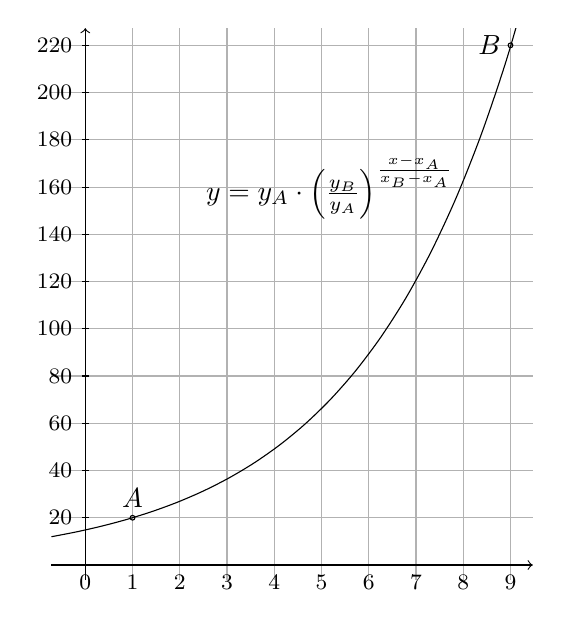
\begin{tikzpicture}[xscale=.6,yscale=.03]
\draw [black!30, xstep=1,ystep=20] (-0.7158634897294093,-6.427853969888794) grid (9.469244912658267,227.24167213330696);
\draw[->] (-0.7158634897294093,0.) -- (9.469244912658267,0.);
\foreach \x in {0,1,2,3,4,5,6,7,8,9}
\draw[shift={(\x,0)}] (0pt,2pt) -- (0pt,-2pt) node[below] {\footnotesize $\x$};
\draw[->] (0.,-6.427853969888794) -- (0.,227.24167213330696);
\foreach \y in {20,40,60,80,100,120,140,160,180,200,220}
\draw[shift={(0,\y)},color=black] (2pt,0pt) -- (-2pt,0pt) node[left] {\footnotesize $\y$};
\clip(-0.7158634897294093,-6.427853969888794) rectangle (9.469244912658267,227.24167213330696);
\draw[smooth,samples=20,domain=-0.7158634897294093:9.469244912658267] plot(\x,{20*(1/11)^((-1)/8*(\x)+1/8)});
\draw[yscale=20,shift={(1,1)}] (0,0) circle (.05) node[above] {$A$};
\draw[yscale=20,shift={(9,11)}] (0,0) circle (.05) node[left] {$B$};
\draw (8,160) node[left]{$y=y_A\cdot\left(\frac{y_B}{y_A} \right)^{\frac{x-x_A}{x_B - x_A}}$};
\end{tikzpicture}
\hfill
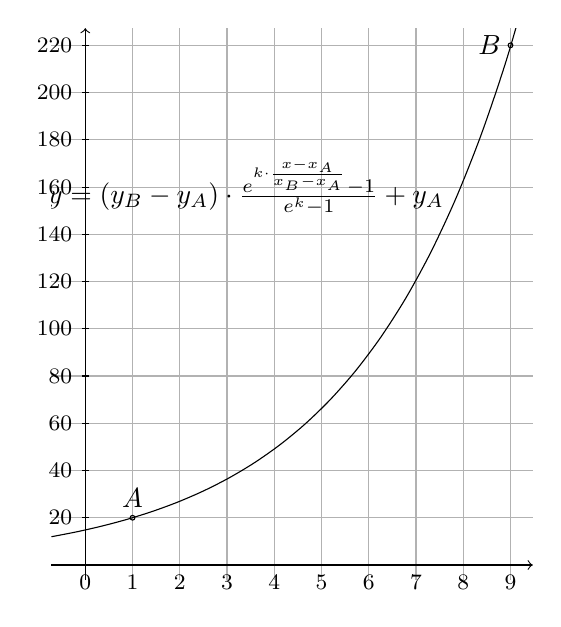
\begin{tikzpicture}[xscale=.6,yscale=.03]
\draw [black!30, xstep=1,ystep=20] (-0.7158634897294093,-6.427853969888794) grid (9.469244912658267,227.24167213330696);
\draw[->] (-0.7158634897294093,0.) -- (9.469244912658267,0.);
\foreach \x in {0,1,2,3,4,5,6,7,8,9}
\draw[shift={(\x,0)}] (0pt,2pt) -- (0pt,-2pt) node[below] {\footnotesize $\x$};
\draw[->] (0.,-6.427853969888794) -- (0.,227.24167213330696);
\foreach \y in {20,40,60,80,100,120,140,160,180,200,220}
\draw[shift={(0,\y)},color=black] (2pt,0pt) -- (-2pt,0pt) node[left] {\footnotesize $\y$};
\clip(-0.7158634897294093,-6.427853969888794) rectangle (9.469244912658267,227.24167213330696);
\draw[smooth,samples=20,domain=-0.7158634897294093:9.469244912658267] plot(\x,{20*(1/11)^((-1)/8*(\x)+1/8)});
\draw[yscale=20,shift={(1,1)}] (0,0) circle (.05) node[above] {$A$};
\draw[yscale=20,shift={(9,11)}] (0,0) circle (.05) node[left] {$B$};
%\draw[yscale=20,shift={(7,6.03)}] (0,0) circle (.05) node[left] {$C$};
\draw (7.8,160) node[left]{$y = (y_B - y_A)\cdot \frac{e^{k\cdot \frac{x - x_A}{x_B - x_A}} - 1}{e^k - 1} + y_A$};
\end{tikzpicture}
}
\end{center}
This function is a special case of a generalized set of functions 
\[y = (y_B - y_A)\cdot \frac{e^{k\cdot \frac{x - x_A}{x_B - x_A}} - 1}{e^k - 1} + y_A\]
depicted in the upper right. This means, when we choose the parameter $k=\ln\left(\frac{y_B}{y_A} \right)$, the upper right function is the same as the upper left function. The great thing about this is, that we can vary now $k$ in order to get similar curves (for $k=0$ we have to use a linear function in order to prevent divison by zero):
\begin{center}
{\small
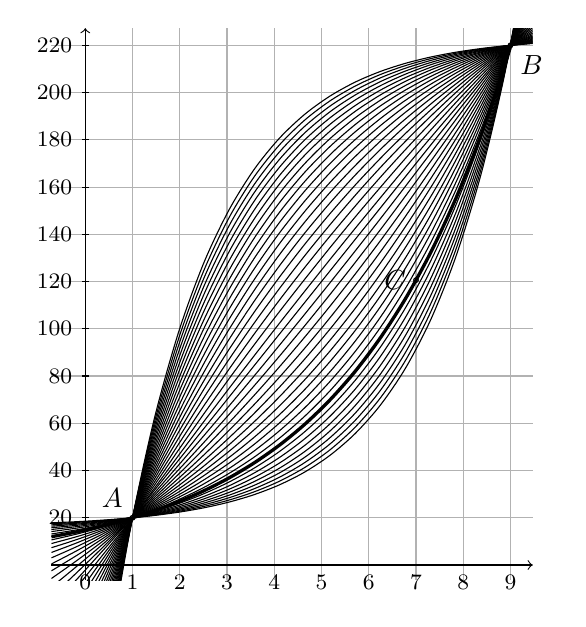
\begin{tikzpicture}[xscale=.6,yscale=.03]
\draw [black!30, xstep=1,ystep=20] (-0.7158634897294093,-6.427853969888794) grid (9.469244912658267,227.24167213330696);
\draw[->] (-0.7158634897294093,0.) -- (9.469244912658267,0.);
\foreach \x in {0,1,2,3,4,5,6,7,8,9}
\draw[shift={(\x,0)}] (0pt,2pt) -- (0pt,-2pt) node[below] {\footnotesize $\x$};
\draw[->] (0.,-6.427853969888794) -- (0.,227.24167213330696);
\foreach \y in {20,40,60,80,100,120,140,160,180,200,220}
\draw[shift={(0,\y)},color=black] (2pt,0pt) -- (-2pt,0pt) node[left] {\footnotesize $\y$};
\clip(-0.7158634897294093,-6.427853969888794) rectangle (10,227.24167213330696);
\foreach \k in {-4,-3.8,...,-.2,.2,.4,...,4}
\draw[smooth,samples=20,domain=-0.7158634897294093:9.469244912658267] plot(\x,{200*(exp(\k* (\x - 1) / 8) - 1) / (exp(\k) - 1) + 20});
\draw[samples=2,domain=-0.7158634897294093:9.469244912658267] plot(\x,{25*\x-5});
\draw[very thick,smooth,samples=20,domain=-0.7158634897294093:9.469244912658267] plot(\x,{20*(1/11)^((-1)/8*(\x)+1/8)});
\draw[yscale=20,shift={(1,1)}] (0,0) circle (.05) node[above left] {$A$};
\draw[yscale=20,shift={(9,11)}] (0,0) circle (.05) node[below right] {$B$};
\draw[yscale=20,shift={(7,6.03)}] (0,0) circle (.05) node[left] {$C$};
%\draw (1,15) node[right]{$y = (y_B - y_A)\cdot \frac{e^{k\cdot \frac{x - x_A}{x_B - x_A}} - 1}{e^k - 1} + y_A$};
\end{tikzpicture}
\hfill
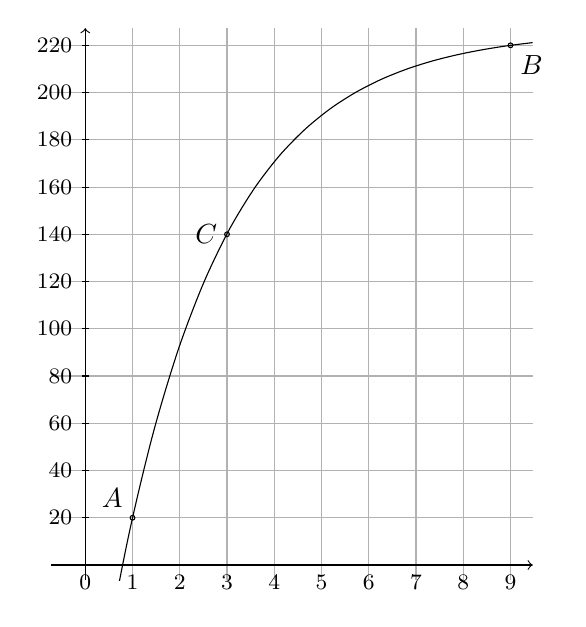
\begin{tikzpicture}[xscale=.6,yscale=.03]
\draw [black!30, xstep=1,ystep=20] (-0.7158634897294093,-6.427853969888794) grid (9.469244912658267,227.24167213330696);
\draw[->] (-0.7158634897294093,0.) -- (9.469244912658267,0.);
\foreach \x in {0,1,2,3,4,5,6,7,8,9}
\draw[shift={(\x,0)}] (0pt,2pt) -- (0pt,-2pt) node[below] {\footnotesize $\x$};
\draw[->] (0.,-6.427853969888794) -- (0.,227.24167213330696);
\foreach \y in {20,40,60,80,100,120,140,160,180,200,220}
\draw[shift={(0,\y)},color=black] (2pt,0pt) -- (-2pt,0pt) node[left] {\footnotesize $\y$};
\clip(-0.7158634897294093,-6.427853969888794) rectangle (10,227.24167213330696);
\draw[smooth,samples=20,domain=-0.7158634897294093:9.469244912658267] plot(\x,{200*(exp(-3.5* (\x - 1) / 8) - 1) / (exp(-3.5) - 1) + 20});
\draw[yscale=20,shift={(1,1)}] (0,0) circle (.05) node[above left] {$A$};
\draw[yscale=20,shift={(9,11)}] (0,0) circle (.05) node[below right] {$B$};
\draw[yscale=20,shift={(3,7)}] (0,0) circle (.05) node[left] {$C$};
\end{tikzpicture}
}
\end{center}
With the generalized function, we can now interpolate three points $A$, $B$ and $C$ --- as long as monotony is still given (depicted in the upper right). Of course, we lose the property of geometric progression. In return, it is now possible that $y$ becomes zero.
\end{document}
